\section{Introdução}

Este trabalho teve como objetivo a implementação e a análise de alguns filtros de imagem no domínio espacial. A filtragem é feita pela convolução da imagem com uma máscara utilizando bibliotecas de processamento de imagens.

A \cref{fig:base} apresenta as imagens base deste trabalho, usadas para análise e discussão dos filtros. Todas elas são monocromáticas. Os filtros utilizados serão apresentados ao longo do relatório, à medida que forem necessários pelo texto.

\begin{figure}[H]
    \centering
    \begin{subfigure}{0.33\textwidth}
    \centering
    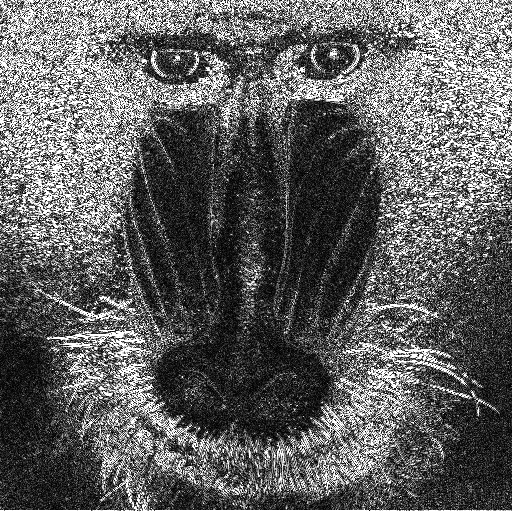
\includegraphics[width=4.4cm]{imagens/baboon.png}
    \caption{\texttt{imagens/baboon.png}}
\end{subfigure}%
\begin{subfigure}{0.33\textwidth}
    \centering
    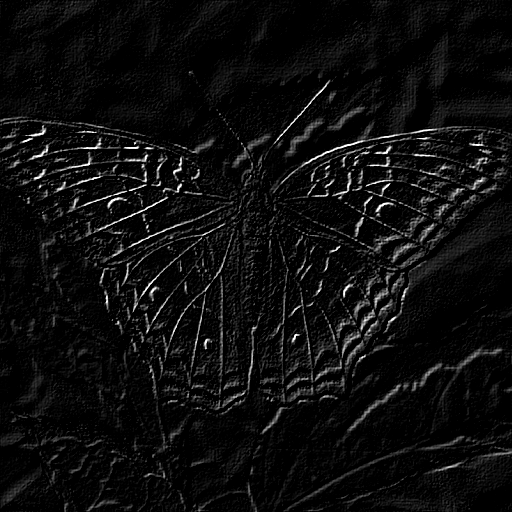
\includegraphics[width=4.4cm]{imagens/butterfly.png}
    \caption{\texttt{imagens/butterfly.png}}
\end{subfigure}\\[8pt]
\begin{subfigure}{0.33\textwidth}
    \centering
    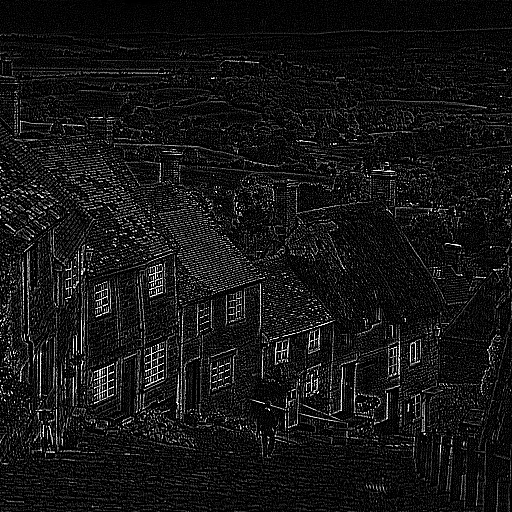
\includegraphics[width=4.4cm]{imagens/city.png}
    \caption{\texttt{imagens/city.png}}
\end{subfigure}%
\begin{subfigure}{0.33\textwidth}
    \centering
    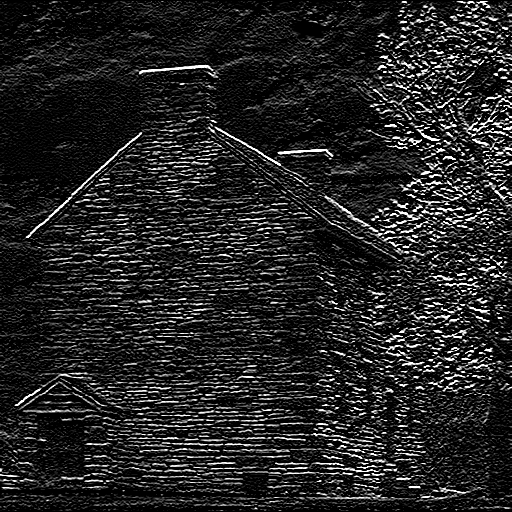
\includegraphics[width=4.4cm]{imagens/house.png}
    \caption{\texttt{imagens/house.png}}
\end{subfigure}%
\begin{subfigure}{0.33\textwidth}
    \centering
    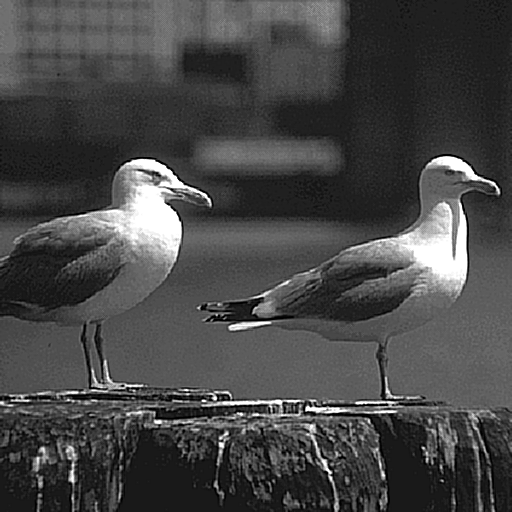
\includegraphics[width=4.4cm]{imagens/seagull.png}
    \caption{\texttt{imagens/seagull.png}}
\end{subfigure}

    \caption{Imagens base da comparação dos filtros.}
    \label{fig:base}
\end{figure}
